%!TEX TS-program = xelatex
%!TEX encoding = UTF-8 Unicode

\documentclass[a4paper,11pt,twoside]{book}
\usepackage{upatras-thesis}
\usepackage{bm}


\newcommand{\shortdoctitle}{Διπλωματική Εργασία}
\newcommand{\doctitle}{Ανάπτυξη συστήματος μεικτής πραγματικότητας για υποστήριξη ατόμων με δυσκολίες όρασης}
\newcommand{\docsubtitle}{Υπότιτλος εγγράφου}
\newcommand{\division}{H/Y}

\newcommand{\me}{Αγγελου Καρδουτσου του Αποστολου}
\newcommand{\metonoi}{Άγγελου Καρδούτσου του Απόστoλου}

\newcommand{\nomme}{Άγγελος Καρδούτσος του Απόστο}

\newcommand{\studnum}{1059372}
\newcommand{\keywords}{keyword1, keyword2, keyword3}
\newcommand{\monthyear}{Οκτώβριος 2023}
\newcommand{\thesisnum}{XXXX}
\newcommand{\supname}{Νικόλαος Αβούρης}
\newcommand{\suptitle} {Καθηγητής}
\newcommand{\headofdivision}{Ονοματεπώνυμο Διεθυντή Τομέα}
\newcommand{\headofdivisiontitle}{Βαθμίδα Διευθυντή Τομέα}

\setlength{\parindent}{24pt}

\author{\me}



% PDF settings
%
\hypersetup
{
    pdfauthor={\me},
    pdftitle={\shortdoctitle},
    pdfsubject={\doctitle},
    pdfkeywords={\keywords},
    pdfproducer={XeLaTex},
    pdfcreator={\creator}
}

\begin{document}


\pagenumbering{roman}
%set the number of sectioning levels that get number and appear in the contents
\setcounter{page}{3}

\begin{titlepage}
\begin{center}
% Upper part of the page
\textsc{\textbf{\large ΠΑΝΕΠΙΣΤΗΜΙΟ ΠΑΤΡΩΝ - ΠΟΛΥΤΕΧΝΙΚΗ ΣΧΟΛΗ}\\
\large ΤΜΗΜΑ ΗΛΕΚΤΡΟΛΟΓΩΝ ΜΗΧΑΝΙΚΩΝ\\ΚΑΙ ΤΕΧΝΟΛΟΓΙΑΣ ΥΠΟΛΟΓΙΣΤΩΝ}\\


\includegraphics[width= 0.8\textwidth]{up_landscape}\\  

\textsc{\Large τομέας: \division }\\[1cm]

\textsc{\uline{\LARGE{\shortdoctitle }}}\\ [0.5cm]
του φοιτητή του Τμήματος Ηλεκτρολόγων Μηχανικών και Τεχνολογίας\\
Υπολογιστών της Πολυτεχνικής Σχολής  του Πανεπιστημίου Πατρών\\[1cm]

\textsc{\LARGE \me }\\[0.5cm]
\textsc{\Large αριθμός μητρώου: \studnum}\\[1cm]

\uline{\large Θέμα}\\[0.5cm]
\textbf{\large \doctitle }\\[1cm]
\uline{\large Επιβλέπων}\\[0.5cm]
\large \supname \\[1cm]
\begin{center}
\large{Αριθμός Διπλωματικής Εργασίας: \thesisnum }\hspace{3cm}
\end{center}
\vfill
% Bottom of the page
\large{Πάτρα, \telosmonthyear}
\end{center}
\end{titlepage}

\clearemptydoublepage

\pagestyle{empty}
\begin{center}
{\LARGE ΠΙΣΤΟΠΟΙΗΣΗ\\[1cm]}
\large Πιστοποιείται ότι η διπλωματική εργασία με θέμα\\[1cm]
\textbf{\bf \large \doctitle }\\[1cm]
του φοιτητή του Τμήματος Ηλεκτρολόγων Μηχανικών και Τεχνολογίας Υπολογιστών\\[1cm]
\textbf{\metonoi}\\[0.5cm]
(Α.Μ.: \studnum)\\[1cm]
παρουσιάστηκε δημόσια στο τμήμα  Ηλεκτρολόγων Μηχανικών και Τεχνολογίας Υπολογιστών στις\\[1cm]
\Large{\imerominiaExetasis}\\[1cm]
\large και εξετάστηκε από την ακόλουθη εξεταστική επιτροπή:\\[1cm]
\supname, \suptitle, \uoP\\[0.2cm]
\epitropiEna, \epitropiEnaTitle, \uoP\\[0.2cm]
\epitropiDyo, \epitropiDyoTitle, \uoP\\[1cm]
\end{center}
\begin{minipage}{0.5\textwidth}
\begin{flushleft} \large
Ο Επιβλέπων\\[0.5cm]
\supname\\
\emph{\suptitle}
\end{flushleft}
\end{minipage}
\begin{minipage}{0.5\textwidth}
\begin{flushright} \large
Ο Διευθυντής του Τομέα\\[0.5cm]
\headofdivision\\
\emph{\headofdivisiontitle}
\end{flushright}
\end{minipage}

\clearemptydoublepage

% !TEX root = ../main.tex

\pagestyle{empty}
\begin{center}
\Large{Στοιχεία διπλωματικής εργασίας}\\[1cm]
{\large Θέμα:}
\textbf{\large \doctitle}\\[1cm]
\large {Φοιτητής: \textbf{\nomme}\\[1cm]
\emph{\large{Ομάδα επίβλεψης}}\\[0.3cm]
\textbf{\supname, \suptitle, \uoP}\\
% \textbf{Βαθμίδα και Ονοματεπώνυμο Συνεπιβλέποντα}\\
% \textbf{\didaktorikosOnoma}\\[1cm]
Περίοδος εκπόνησης της εργασίας:\\ {\arximonthyear} - {\telosmonthyear}\\[1cm]
Η εργασία αυτή γράφτηκε στο \XeLaTeX{} και χρησιμοποιήθηκε η γραμματοσειρά GFS Didot του Greek Font Society.}
\end{center}

\clearemptydoublepage

\pagestyle{plain}
\begin{center}
{\LARGE Περίληψη}\\[1cm]
\end{center}

\setlength{\parindent}{0pt}
\textbf{Παράγραφος 1}: Περιγραφή σκοπού διπλωματικής

\textbf{Παράγραφος 2}: Περιγραφή του τι περιγράφουμε στο τεχνολογικό υπόβαθρο και για
την ανάπτυξη της εφαρμογής

\textbf{Παράγραφος 3}: Περιγραφή του πειράματος (τόπος και τρόπος διεξαγωγής, συμμετέχοντες)

\textbf{Παράγραφος 4}: Περογραφή του τελευταίου κεφαλαίου

\textbf{Λέξεις-κλειδιά}: {\keywords}


\clearemptydoublepage

\begin{center}
{\LARGE Ευχαριστίες}\\[1cm]
\end{center}

\setlength\parindent{24pt}Όσο κι αν φαίνεται σαν ατομική δουλειά η παρούσα εργασία, στην πραγματικότητα βοήθησαν αρκετοί άνθρωποι (ο καθένας με το δικό του τρόπο) για να ολοκληρωθεί. 

\clearemptydoublepage

\pagestyle{fancy}

\tableofcontents
\clearemptydoublepage
\listoffigures
\clearemptydoublepage
\listoftables
\clearemptydoublepage

%\mainmatter % book mode only

\pagenumbering{arabic}
\setcounter{page}{1}

%!TEX root = ../main.tex

\chapter*{Εισαγωγή}
\markboth{Εισαγωγη}{}
%\vspace{-1.3in}
\lettrine[findent=2pt]{\fbox{\textbf{Η}}}{εργασια} αυτή έχει γίνει προσπάθεια να γραφεί σε ανεξάρτητα κεφάλαια, τα οποία θα δώσουν στον αναγνώστη τις απαιτούμενες γνώσεις ώστε να καταλάβει σε βάθος τις τεχνικές που χρησιμοποιούνται. Σε κάθε κεφάλαιο γίνεται αναλυτική παρουσίαση των τεχνικών καθώς και του υπόβαθρου που πρέπει να έχει κάποιος ώστε τις κατανοήσει, ωστόσο θεωρείται πως ο αναγνώστης έχει ήδη κάποιες γνώσεις στο χώρο της επεξεργασίας σήματος και εικόνας. Έτσι, βασικές έννοιες και μηχανισμοί της ανωτέρω περιοχής θα θεωρούνται δεδομένοι και δε θα γίνει κάποια ανάλυσή τους στο κείμενο αυτό, εκτός αν κρίνεται απαραίτητο.

\clearemptydoublepage

\chapter{Θεωρητικό και Τεχνολογικό Υπόβαρο}\label{ch:chap2}
{\LARGE ΘΕΩΡΙΑ}\\
Blindness
- Temporary solutions
- Accessibility
Extended reality
Hololens
- Description of the device
Hololens features
Unity
%!TEX root = ../main.tex



\section{Η υπέρυθρη ακτινοβολία}

\begin{figure}
  \centering
  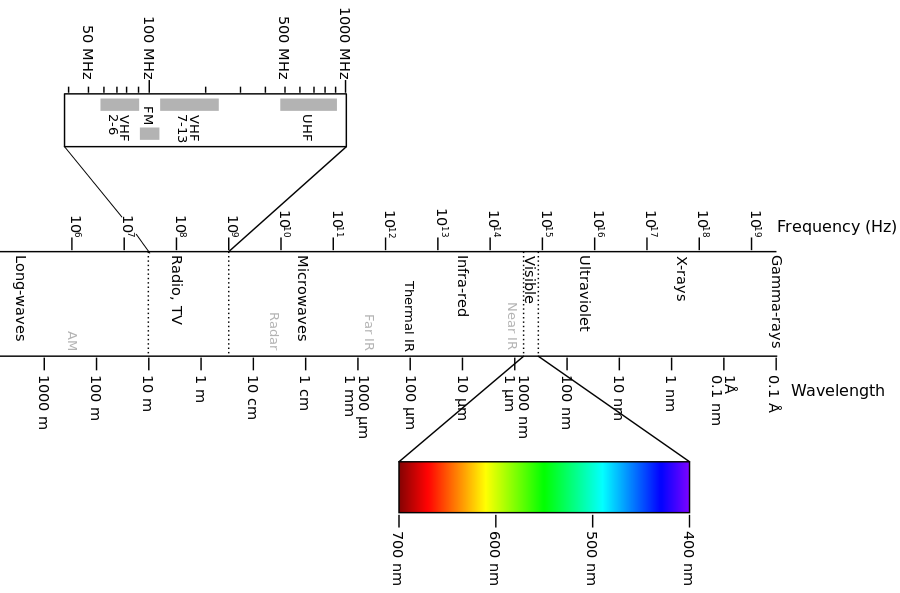
\includegraphics[width=\textwidth]{spectrum}
  \caption{Το φάσμα της Ηλεκτρομαγνητικής Ακτινοβολίας}
  \label{fig:spectrum}
\end{figure}


\lettrine[findent=2pt]{\fbox{\textbf{Ό}}}{πως} γνωρίζουμε από την επιστήμη της Φυσικής, όταν ένα σώμα ζεσταθεί αρκετά (π.χ. > 100 C) αρχίζει και εκπέμπει ακτινοβολία και στο οπτικό φάσμα (πέραν του υπέρυθρου), ενώ αποκτά ταυτόχρονα μια ερυθρή όψη. Κατά το φαινόμενο αυτό, η ακτινοβολια που εκπέμπεται ανήκει τόσο στο υπέρυθρο, όσο και στο ορατό φάσμα της ηλεκτρομαγνητικής ακτινοβολίας και μάλιστα το χρώμα που αποκτά το σώμα συνδέεται άμεσα με τη θερμοκρασία στην οποία βρίσκεται. Οι περιοχές της υπέρυθρης και ορατής ακτινοβολίας, καταλαμβάνουν τις ζώνες $1mm - 700nm$ και $700nm - 390nm$ αντίστοιχα, όπως φαίνεται και στο σχήμα \ref{fig:spectrum}.
\clearemptydoublepage

\chapter{Η υλοποίηση}\label{ch:chap3}
{\LARGE ΥΛΟΠΟΙΗΣΗ}\\

%!TEX root = ../main.tex

Σκοπός του κεφαλαίου αποτελεί η παρουσίαση της διαδικασίας ανάπτυξης της εφαρμογής για τη συσκευή Microsoft HoloLens 2. Πιο συγκεκριμένα, θα παρουσιάσουμε αρχικά τον κύριο στόχο της εφαρμογής, ποιος είναι ο σκοπός που εξυπηρέτει και σε ποιο πρόβλημα προσπαθεί να προσφέρει λύση (\hyperref[sec:appScenario]{Κεφάλαιο~\ref*{sec:appScenario}}). Έπειτα, θα γίνει αναφορά στις αποφάσεις που λήφθηκαν κάτα την σχεδίαση και υλοποίηση της εφαρμογής με βάση και τους περιορισμούς που τέθηκαν (\hyperref[sec:appDesignAndLimitations]{Κεφάλαιο~\ref*{sec:appDesignAndLimitations}}), ενώ θα δοθεί και μια αναλυτική περιγραφή της διαδικασίας υλοποίησης της εφαρμογής και επεξήγηση του κώδικα που αναπτύχθηκε (\hyperref[sec:appImplementation]{Κεφάλαιο~\ref*{sec:appImplementation}}). Το κεφάλαιο θα ολοκληρωθεί παρουσιάζοντας όλες τις κύριες λειτουργίες, οι οποίες αναπτύχθηκαν για την εφαρμογή (\hyperref[sec:appFunctionalities]{Κεφάλαιο~\ref*{sec:appFunctionalities}}).

%TODO: Εναλλακτικός τίτλος: Περιγραφή/Λειτουργίες Εφαρμογής
\section{Σενάριο Εφαρμογής}\label{sec:appScenario}
Στόχος εφαρμογής\\
Περιγραφή σεναρίου χρήσης εφαρμογής

\section{Σχεδιασμός και Περιορισμοί}\label{sec:appDesignAndLimitations}
Κατά τον σχεδιασμό της εφαρμογής, καθώς και κατά τη διάρκεια υλοποίησης αυτής, υπήρξαν πληθώρα περιπτώσεων, όπου κληθήκαμε να λάβουμε ιδιαίτερα σημαντικές αποφάσεις, που επηρέασαν σημαντικά την πορεία ανάπτυξης, λόγων των συνθηκών και προδιαφραφών που τέθηκαν ή των περιορισμών και δυσκολιών που αντιμετωπίσαμε.

Αρχικά, όσον αφορά την προετοιμασία και την εγκατάσταση των εργαλείων, ήρθαμε αντιμέτωποι με ένα ιδιαίτερα λειψό εγχειρίδιο (documentation)~\cite{hferrone_mixed}, το οποίο παρέχει η Microsoft.
Ειδικότερα, το documentation είναι πλούσιο σε πληροφοριές, που βοηθούν προγραμματιστές, οι οποίοι έρχονται πρώτη φορά σε επαφή με το headset, να κατανοήσουν πλήρως έννοιες και τεχνολογίες που αξιοποοιούνται από τη συσκευή, καθώς και τον τρόπο λειτουργίας της. Ωστόσο, σε προγραμματιστικό επίπεδο, οι πληροφορίες είναι ελάχιστες, ενώ οι επεξηγήσεις αντικειμένων, κλάσεων και συναρτήσεων είναι ιδιαίτερα ελλιπείς, καθώς περιορίζονται σε επιδερμικές περογραφές αυτών και την παρουσιασή παραδειγμάτων και σε ένα πολύ μικρό δείγμα αυτών.
Παράλληλα, η Microsoft παρέχει μαθήματα (courses) για την πρακτική εκμάθηση των προγραμματιστών στην ανάπτυξη εφαρμογών για τη συσκεύη με τη χρήση του περιβάλλοντος Unity. Όμως, και σε αυτή την περίπτωση, τα courses περιορίζονται στη χρήση έτοιμων projects, όπου η μόνη συμβολή του χρήστη στη ανάπτυξη αυτών είναι η αλλαγή ορισμένων απλών ρυθμίσεων. Επομένως, κατά τη διάρκεια της ανάπτυξης (development), αναγκαστήκαμε να καταφύγουμε σε οδηγούς (tutorials) και forums, τα οποία αναπτύχθηκαν από τρίτους, από κοινότητες προγραμματιστών που διέθεταν εμπειρία πάνω στη συγκεκριμένη τεχνολογία.
Τέλος, ιδιαίτερο πρόβλημα αποτέλεσε η ασυμβατότητα (incompatibility) μεταξύ των διαφορετικών εκδόσεων των εργαλείων που χρησιμοποιήθηκαν (Unity, MRTK, Visual Studio), το οποίο καθυστέρησε την έναρξη της φάσης ανάπτυξης (development phase).

Επιπλέον, λόγω της ιδιαιτερότητας των χρηστών προς τους οποίους απευθύνεται η εφαρμογή, εκ πρώτης όψεως, φαίνεται αρκέτα οξύμωρη η επιλογή μίας συσκευής που ενσωματώνει την τεχνολογία Μικτής Πραγματικότητας, όπου, επί τον πλείστον, οι εφαρμογές απαιτούν από τους χρήστες να αλληλεπιδράσουν με εικονικά αντικείμενα και η όραση αποδεικνύεται εξαιρετικά σημαντική. Παρ' όλα αυτά, η συσκευή επιλέχθηκε λόγω compact σχεδιασμού, ενσωματώνοντας πληθώρα αισθητήρων σε μια μικρή, φορητή συσκευή. Επίσης, ο προγραμματιστής έχει τη δυνατότητα να ενσωματώσει φωνητικές εντολές, όπου οι χρήστες μπορούν χρησιμοποιήσουν για να αλληλεπιδράσουν με τις λειτουργίες της εφαρμογής.

Πέρα από τις δυνατότητες που προσφέρει η συσκευή, καθιστώντας την ιδανική επιλογή, θέτει, παράλληλα, έχει και ορισμένους περιορισμούς. Συγκεκριμένα, οι περιορισμοί αφορούν τις συνθήκες του περιβάλλοντος, όπου χρησιμοποιείται η συσκευή~\cite{dorreneb_2022_hololens}. 
Για την αποδοτική λειτουργία της συσκευής, πρέπει ο χώρος να είναι καλά φωτιζόμενος, να μην είναι ιδιαίτερα απλός, αλλά, αντιθέτως, να διαθέτει πολλά, μοναδικά αντικειμένα, τα οποία θα εξυπηρετήσουν στην καλύτερη αναγνώριση των αντικειμένων και των εμποδίων κατά τη χωρική χαρτογράφηση. Τέλος, οι συχνές αλλαγές και μετακινήσεις στο χώρο, καθώς και η ύπαρξη ανακλαστικών επιφανειών μπορούν να επηρεάσουν αρνητικά το tracking και τη χαρτογράφηση της συσκευής.
Για τους ανωτέρω λόγους, αποφασίστηκε η χρήση της εφαρμογής να περιοριστεί σε εσωτερικούς χώρους.

% Αδυναμία ανθρώπου να αντιληφθεί προέλευση ήχου στον κάθετο άξονα

\section{Υλοποίηση}\label{sec:appImplementation}
Η υλοποίηση της εφαρμογής, τμηματοποιημένη

\section{Λειτουργίες Εφαρμογής}\label{sec:appFunctionalities}
Τρόπος χρήσης της εφαρμογής

% \begin{theorem}[Shannon-Nyquist]
% 	\label{thrm:shannon-nyquist}
% 	Ένα σήμα με μέγιστη συχνότητα $f_{max}$ μπορεί να ανακτηθεί από τα δείγματά του, αν αυτά ληφθούν με συχνότητα $f_s>2f_{max}$, ή αλλιώς με περίοδο $T_s<\frac{1}{2f_{max}}$. \cite{proakis_sampling}
% \end{theorem}
\clearemptydoublepage

\chapter{Αξιολόγηση}\label{ch:chap4}
{\LARGE ΑΞΙΟΛΟΓΗΣΗ}\\
\clearemptydoublepage

\chapter{Αποτελέσματα}\label{ch:chap5}
{\LARGE ΑΠΟΤΕΛΕΣΜΑΤΑ ΑΞΙΟΛΟΓΗΣΗΣ ΚΑΙ ΣΧΟΛΙΑ}\\
\clearemptydoublepage

\chapter{Μελλοντικές Εφαρμογές}\label{ch:chap6}
{\LARGE ΒΕΛΤΙΩΣΕΙΣ ΚΑΙ ΠΡΟΕΚΤΑΣΕΙΣ}\\

%!TEX root = ./main.tex

\begin{thebibliography}{99}

\bibitem{c1} S. C. Park, M. K. Park, and M. G. Kang, “Super-resolution image reconstruction:
A technical overview,” IEEE Signal Processing Magazine, vol. 20, no. 3, pp. 21–36,
May 2003.
\bibitem{keren} D. Keren, S. Peleg, and R. Brada, “Image sequence enhancement using subpixel
displacements,” in IEEE Computer Society Conference on Computer Vision and
Pattern Recognition, June 1988, pp. 742–746.
\bibitem{hardie} R. Hardie, K. Barnard, and E. Armstrong, “Joint MAP registration and high resolution image estimation using a sequence of undersampled images,” IEEE Transactions on Image Processing, vol. 6, no. 12, pp. 1621–1633, December 1997.
\bibitem{patti} A. Patti, M. Sezan, and A. Tekalp, “High-resolution image reconstruction from
a low-resolution image sequence in the presence of time-varying motion blur,” in
Proceedings of the IEEE International Conference on Image Processing, Austin,
TX, vol. 1, 1994, pp. 343–347.
\bibitem{hardie2} R. C. Hardie, K. J. Barnard, J. G. Bognar, E. E. Armstrong, and E. A. Watson, “High resolution image reconstruction from a sequence of rotated and translated
frames and its application to an infrared imaging system,” Optical Engineering,
vol. 37, no. 1, pp. 247–260, January 1998.
\bibitem{alam} M. S. Alam, J. G. Bognar, R. C. Hardie, and B. J. Yasuda, “Infrared image registration and high-resolution reconstruction using multiple translationally shifted aliased video frames,” IEEE Transactions on Instrumentation and Measurement, vol. 49,
no. 5, pp. 923–915, October 2000.
\bibitem{tsai} R. Y. Tsai and T. S. Huang, “Multiframe image restoration and registration,” in Advances in Computer Vision and Image Processing: Image Reconstruction from Incomplete Observations, T. S. Huang, Ed., vol. 1. London: JAI Press, 1984, pp. 317–339.
\bibitem{kim} N. K. Bose, H. C. Kim, and H. M. Valenzuela, “Recursive total least squares algorithm for image reconstruction from noisy undersampled frames,” Multidimensional Systems and Signal Processing, vol. 4, no. 3, pp. 253–268, July 1993.
\bibitem{yang} J. Yang, J. Wright, T. Huang, and Yi Ma. Image super-resolution via sparse representation. IEEE Transactions on Image Processing (TIP), vol. 19, issue 11, 2010.
\bibitem{ransac} Martin A. Fischler and Robert C. Bolles (June 1981). “Random Sample Consensus: A Paradigm for Model Fitting with Applications to Image Analysis and Automated Cartography”. Comm. of the ACM 24 (6): 381–395
\bibitem{wired_ff_algo} Jordan Ellenberg, ”Fill in the Blanks: Using Math to Turn Lo-Res Datasets Into Hi-Res Samples”, 22 February 2010, Wired Magazine \url{http://www.wired.com/2010/02/ff_algorithm/}
\bibitem{incoherence} D.L. Donoho and X. Huo, “Uncertainty principles and ideal atomic decomposition,” IEEE Trans. Inform. Theory, vol. 47, no. 7, pp. 2845–2862, Nov. 2001.
\bibitem{candes} E. Candes, “Compressive sensing,” in Proceedings of the International Congress of Mathematicians, vol. 3, pp. 1433–1452, 2006.
\bibitem{donoho} D. L. Donoho, “Compressed sensing,” IEEE Transactions on Information Theory, vol. 52, no. 4, pp. 1289–1306, 2006.
\bibitem{proakis_sampling} John G. Proakis, Dimitris G. Manolakis , “Digital Signal Processing - Principles, Algorithms, Implementations” 4th edition (Pearson International Edition), Pearson Education, Chapter 1.4.2: The Sampling Theorem 
\bibitem{gonzalez_2d_fft} Rafael C. Gonzalez, Richard E. Woods , “Digital Image Processing” 3rd edition (Pearson International Edition), Pearson Education, Chapter 1.4.2: The 2D Discrete Fourier Transform and its Inverse
\bibitem{shift_add_fusion} S. Farsiu, M. Elad, P. Milanfar, “Fast and Robust Multiframe Super Resolution” IEEE Transactions on Image Processing, vol. 13, no. 10, October 2004
\bibitem{imregintro} ”Image Registration", in Wikipedia: The Free Encyclopedia; (Wikimedia Foundation Inc., updated 2 December 2014, 15:50 UTC) \url{http://en.wikipedia.org/wiki/Image_registration}
\bibitem{cs_intro} M. Davenport, M. Duarte, Y. Eldar, G. Kutyniok, ”Introduction to Compressed Sensing”, Stanford University - Department of Statistics
\bibitem{convexmin} F. Bach, R. Jenatton, J. Mairal, G. Obozinski, ”Convex Optimization with Sparsity-Inducing Norms”, Institut National de Recherche en Informatique et en Automatique (INRIA)
\bibitem{red_dict} H. Rauhut, K. Schnass, and P. Vandergheynst, “Compressed sensing and redundant dictionaries,” IEEE Transactions on Information Theory, vol. 54, no. 5, May 2008.
\bibitem{denoising_dict} M. Elad and M. Aharon, “Image denoising via sparse and redundant representations over learned dictionaries,” IEEE Transactions on Image Processing, vol. 15, pp. 3736–3745, 2006.
\bibitem{im_vid_rest} J. Mairal, G. Sapiro, and M. Elad, “Learning multiscale sparse representations for image and video restoration,” Multiscale Modeling and Simulation, vol. 7, pp. 214–241, 2008.
\bibitem{ksvd_dict} M. Aharon, M. Elad, and A. Bruckstein, “K-SVD: An algorithm for designing overcomplete dictionaries for sparse representation,” IEEE Transactions on Signal Processing, vol. 54, no. 11, pp. 4311–4322, Nov. 2006.
\bibitem{sparse_coding_dict} H. Lee, A. Battle, R. Raina, and A. Y. Ng, “Efficient sparse coding algorithms,” in Advances in Neural Information Processing Systems (NIPS), pp. 801–808, 2007.
\bibitem{human_sparse} B. Olshausen and D. Field, “Sparse coding with an overcomplete basis set: A strategy employed by V1?,” Vision Research, vol. 37, no. 23, pp. 3311–3325, 1997.
\bibitem{nphard} ”NP-hard", in Wikipedia: The Free Encyclopedia; (Wikimedia Foundation Inc., updated 9 April 2015, 15:30 UTC) \url{http://en.wikipedia.org/wiki/NP-hard}
\bibitem{nphard1} D. L. Donoho, “For most large underdetermined systems of linear equations, the minimal $l_1$-norm solution is also the sparsest solution,” Communications on Pure and Applied Mathematics, vol. 59, no. 6, pp. 797–829, 2006.
\bibitem{nphard2} “For most large underdetermined systems of linear equations, the minimal $l_1$-norm near-solution approximates the sparsest near-solution,” Communications on Pure and Applied Mathematics, vol. 59, no. 7, pp. 907–934, 2006.
\bibitem{lasso} R. Tibshirani, “Regression shrinkage and selection via the lasso,” Jour- nal of Royal Statistical Society, Series B, vol. 58, no. 1, 1996.
\bibitem{dict_training} Jianchao Yang, Zhaowen Wang, Zhe Lin, and Thomas Huang. Coupled dictionary training for image super-resolution. IEEE Transactions on Image Processing (TIP), vol. 21, issue 8, pages 3467-3478, 2012.
\bibitem{srexample} W. T. Freeman, T. R. Jones, and E. C. Pasztor, “Example-based superresolution,” IEEE Computer Graphics and Applications, vol. 22, pp. 56–65, 2002.
\bibitem{lowlevel} W. T. Freeman, E. C. Pasztor, and O. T. Carmichael, “Learning low-level vision,” International Journal of Computer Vision, vol. 40, no. 1, pp. 25–47, 2000.
\bibitem{sr_neigh} H. Chang, D.-Y. Yeung, and Y. Xiong, “Super-resolution through neighbor embedding,” in IEEE Conference on Computer Vision and Pattern Classifi- cation (CVPR), vol. 1, pp. 275–282, 2004.
\bibitem{imhal} J. Sun, N. N. Zheng, H. Tao, and H. Shum, “Image hallucination with primal sketch priors,” in IEEE Conference on Computer Vision and Pattern Recognition (CVPR), vol. 2, 2003, pp. 729–736.
\bibitem{imfill} imfill, Image Processing Toolbox Documentation, MathWorks \\ \url{http://www.mathworks.com/help/images/ref/imfill.html}
\bibitem{imresize} imresize, Image Processing Toolbox Documentation, MathWorks \\ \url{http://www.mathworks.com/help/images/ref/imresize.html}
\bibitem{k-term} A. Cohen, W. Dahmen, R. DeVorce, "Compressed sensing and best k-term approximation", in the Journal of the American Mathematical Society, vol. 22, pp. 211-231 , 2009.




\end{thebibliography}

\clearemptydoublepage

\pagestyle{empty}

\vspace*{\fill}
%\hline
\begin{flushleft}
	Πανεπιστήμιο Πατρών, Πολυτεχνική Σχολή \\
	Τμήμα Ηλεκτρολόγων Μηχανικών και Τεχνολογίας Υπολογιστών \\
	{\nomme} \\
	© \telosmonthyear \ -- Με την επιφύλαξη παντός δικαιώματος.\\
\end{flushleft}
%\hline


\end{document}
